% Канонический TikZ-рисунок варианта 24. Править только здесь.
\newcommand{\figCyclicTwoAngles}{%
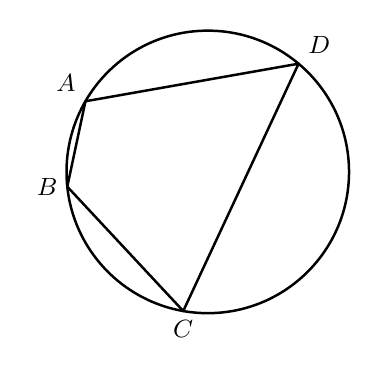
\begin{tikzpicture}[scale=0.78,line cap=round,line join=round,every node/.style={font=\small}]
  \def\R{2.3}
  \coordinate (A) at (150:\R); \coordinate (B) at (186:\R);
  \coordinate (C) at (260:\R); \coordinate (D) at (50:\R);
  \draw[line width=0.9pt] (0,0) circle (\R);
  \draw[line width=0.9pt] (A)--(B)--(C)--(D)--cycle;
  \node[above left] at (A) {\(A\)}; \node[left] at (B) {\(B\)};
  \node[below] at (C) {\(C\)}; \node[above right] at (D) {\(D\)};
\end{tikzpicture}}
